\chapter{Cronograma}
%\begin{figure}[H]
%	\centering
%	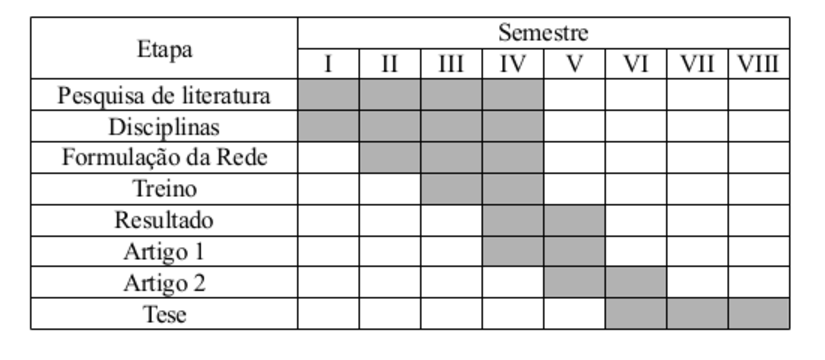
\includegraphics[height=6.5cm, width=16cm]{Imagens/Cronograma.pdf}
%	\caption{Cronograma previsto para o projeto.}
%\end{figure}

Em  {\color{red}vermelho} encontra-se o mês atual.
\begin{table}[H]
	\centering
	%\flushleft
	
	% definindo o tamanho da fonte para small
	% outros possíveis tamanhos: footnotesize, scriptsize
	\begin{small}
		
		% redefinindo o espaçamento das colunas
		\setlength{\tabcolsep}{2pt}
		
		% \cline é semelhante ao \hline, porém é possível indicar as colunas que terão essa a linha horizontal
		% \multicolumn{10}{c|}{Meses} indica que dez colunas serão mescladas e a palavra Meses estará centralizada dentro delas.
		\rotatebox{0}{
			\begin{tabular}{|c|c|c|c|c|c|c|c|c|c|c|c|c|c|c|c|c|c|c|c|c|c|c|c|c|}\hline
				& \multicolumn{24}{c|}{Meses}\\ \cline{2-25}
				\raisebox{1.5ex}{Etapa} & 01 & 02 & 03 & 04 & 05 & 06 & 07 & 08 & {\color{red}09} & 10 & 11 & 12 & 13 & 14 & 15 & 16 & 17 & 18 & 19 & 20 & 21 & 22 & 23 & 24 \\ \hline
				
				Pesquisa na Literatura & X & X & X & X & X & X & X & X & {\color{red}X} & X & X & X & X & X & X & X & X & X & X & X & X & X & X & X\\ \hline
				Disciplinas & & & X & X & X & X & X & X &  {\color{red}X} & X & X & X & & & X & X & X & X & X & X & X & X & X & X \\ \hline
				Formulação da Rede & & & & & & & & X &  {\color{red}X} & X & X & X & X & X & X & X & & & & & & & \\ \hline
				Treino & & & & & & & & & & & & & X & X & X & X & X & X & X & X & X & X & X & X \\ \hline
				Resultado & & & & & & & & & & & & & & & & & & & & X & X & X & X & X \\ \hline
				Artigo 1 & & & & & & & & & & & & & & & & & & & & & & & X & X \\ \hline
				Artigo 2 & & & & & & & & & & & & & & & & & & & & & & & & \\ \hline
				Tese & & & & & & & & & & & & & & & & & & & & & & & & \\ \hline
			\end{tabular}
		}
	\end{small}
	\caption{Cronograma das atividades previstas para o primeiro biênio.}
	\label{t1_cronograma}
\end{table}


\begin{table}[H]
	\centering
	
	% definindo o tamanho da fonte para small
	% outros possíveis tamanhos: footnotesize, scriptsize
	\begin{small}
		
		% redefinindo o espaçamento das colunas
		\setlength{\tabcolsep}{2pt}
		
		% \cline é semelhante ao \hline, porém é possível indicar as colunas que terão essa a linha horizontal
		% \multicolumn{10}{c|}{Meses} indica que dez colunas serão mescladas e a palavra Meses estará centralizada dentro delas.
		\rotatebox{0}{
			\begin{tabular}{|c|c|c|c|c|c|c|c|c|c|c|c|c|c|c|c|c|c|c|c|c|c|c|c|c|}\hline
				& \multicolumn{24}{c|}{Meses}\\ \cline{2-25}
				\raisebox{1.5ex}{Etapa} & 25 & 26 & 27 & 28 & 29 & 30 & 31 & 32 & 33 & 34 & 35 & 36 & 37 & 38 & 39 & 40 & 41 & 42 & 43 & 44 & 45 & 46 & 47 & 48 \\ \hline
				
				Pesquisa na Literatura & X & X & X & X & X & X & & & & & & & & & & & & & & & & & & \\ \hline
				Disciplinas & & & & & & & & & & & & & & & & & & & & & & & & \\ \hline
				Formulação da Rede & & & & & & & & & & & & & & & & & & & & & & & & \\ \hline
				Treino & & & & & & & & & & & & & & & & & & & & & & & & \\ \hline
				Resultado & & X & X & X & X & X & X & X & & & & & & & & & & & & & & & & \\ \hline
				Artigo 1 & & X & X & X & & & & & & & & & & & & & & & & & & & & \\ \hline
				Artigo 2 & & & & & X & X & X & X & X & & & & & & & & & & & & & & & \\ \hline
				Tese & & & & & & & & & & & & & & & X & X & X & X & X & X & X & & & \\ \hline
				
			\end{tabular}
		}
	\end{small}
	\caption{Cronograma das atividades previstas para o segundo biênio.}
	\label{t2_cronograma}
\end{table}